\section{Introduction}

Thermal reflow processes can significantly modify the profile obtained in polymer resist and this phenomenon has its advantages and disadvantages.
For example, thermal reflow is applied as a stage of microfabrication for smoothing of the relief obtained by grayscale e-beam lithography~\cite{Kirchner_GL_review} or nanoimprint lithography~\cite{NIL_reflow}, which allows one to obtain various 3D structures.
On the other hand, resist profile deformation by thermal reflow reduces profile aspect ratio, which is undesirable in certain cases. Thermal reflow can also affect structures obtained by standard ``wet'' e-beam lithography process.
E-beam exposure and proximity effects lead to molecular weight reduction of the whole resist layer, which stimulates resist reflow at post-exposure and post-develop bake stages.
In the light of the foregoing, the method allowing exact determination of reflow processes influence on resulting structure profile in any specific processes is highly desirable.

Two common approaches to simulation of resist thermal reflow could be distinguished. The first include analytical methods based on transfer equations. For instance, Leveder et al. used an analytical spectral method to simulate the reflow of isodense periodic structures with various periods~\cite{Leveder_2008, Leveder_2010, Leveder_2011}. This method is based on 2D Navier-Stokes equation coupled to continuity equation with the assumption of no slip length and no Marangoni effect but considering Laplace pressure and Hamaker energy. In this algorithm the initial structure profile is Fourier transformed and then reflow process is simulated by decay of profile harmonics:
\begin{eqnarray} \label{eq:Fourier}
	h(x, t) = h_0 + \tilde{h}(x, t),\\
	\tilde{h}(x, t) = \sum_{-\infty}^{+\infty} a_n(0) \exp \left(-\frac{t}{\tau_n}+i n \frac{2 \pi}{\lambda} x \right),\\
	\tau_n = \frac{3 \eta}{\gamma h_0^3} \times \left( \frac{\lambda}{2 \pi n} \right)^4,
\end{eqnarray}
where $\lambda$ -- profile spatial periodicity, $\eta$, $\gamma$ -- polymer viscosity and surface tension, respectively, $a_n(0)$ -- Fourier coefficients of initial polymer profile, $h_0$ -- polymer layer thickness. Polymer viscosity depends both on temperature and polymer molecular weight, which should be taken into account in simulation. Temperature dependence of viscosity could be described by Williams–Landel–Ferry (WLF) equation~\cite{bird1987dynamics_WLF}:

\begin{equation} \label{eq:WLF}
	\log \left( \frac{\eta(T)}{\eta(T_0)} \right) = -\frac{C_1(T-T_0)}{C_2+(T-T_0)},
\end{equation}
which parameters $\eta(T_0)$, $C_1$, $C_2$ and $T_0$ for three different resists are provided in Table~\ref{table:WLF}~\cite{aho2008_measurement_WLF}.

\begin{table}[h]
	\centering
	\caption{Parameters of equation~\ref{eq:WLF}, obtained by Aho et al. for polystyrene 143E by BASF (PS), poly(methyl methacrylate) Plexiglas 6N by Degussa (PMMA) and polycarbonate Lexan HF1110R by GE Plastics (PC)~\cite{aho2008_measurement_WLF}.}
	\begin{tabular}{l l l l}
		\br
		Parameter \hspace{8.9em} & PS \hspace{5em} & PMMA \hspace{5em} & PC \\
		\mr
		$\eta(T_0)$, Pa$\cdot$s \hspace{8.9em} & 7310.4 \hspace{5em} & 13450 \hspace{5em} & 2763 \\
		$C_1$ \hspace{8.9em} & 10.768 \hspace{5em} & 7.6682 \hspace{5em} & 4.7501 \\
		$C_2$, $^\circ$C \hspace{8.9em} & 289.21 \hspace{5em} & 210.76 \hspace{5em} & 110.12 \\
		$T_0$, $^\circ$C \hspace{8.9em} & 190 \hspace{5em} & 200 \hspace{5em} & 200 \\
		\br
	\end{tabular}
	\label{table:WLF}
\end{table}

\noindent Withal, the dependence of polymer viscosity on its molecular weight could be described by empirical formula:

\begin{equation} \label{eq:3p4_3p1}
	\eta \propto M_n^\alpha,
\end{equation}
where $M_n$ -- number average polymer molecular weight. For PMMA $\alpha$ comprises 3.4 at $M_n \geq 48 000$ and 1.4 at $M_n < 48 000$~\cite{Leveder_2010, Bueche_3p4_1p4}. Equations~(\ref{eq:WLF}, \ref{eq:3p4_3p1}) allow one to calculate polymer viscosity for different temperatures and molecular weights (Fig.~\ref{fig:eta_vary_T_Mn}). The accuracy of this analytical method is quite high for the simulation of polymer reflow at $a_n(t) \ll h_0$, however, it couldn't be applied in case of non-uniform polymer viscosity profile.

\begin{figure}
	\begin{center}
		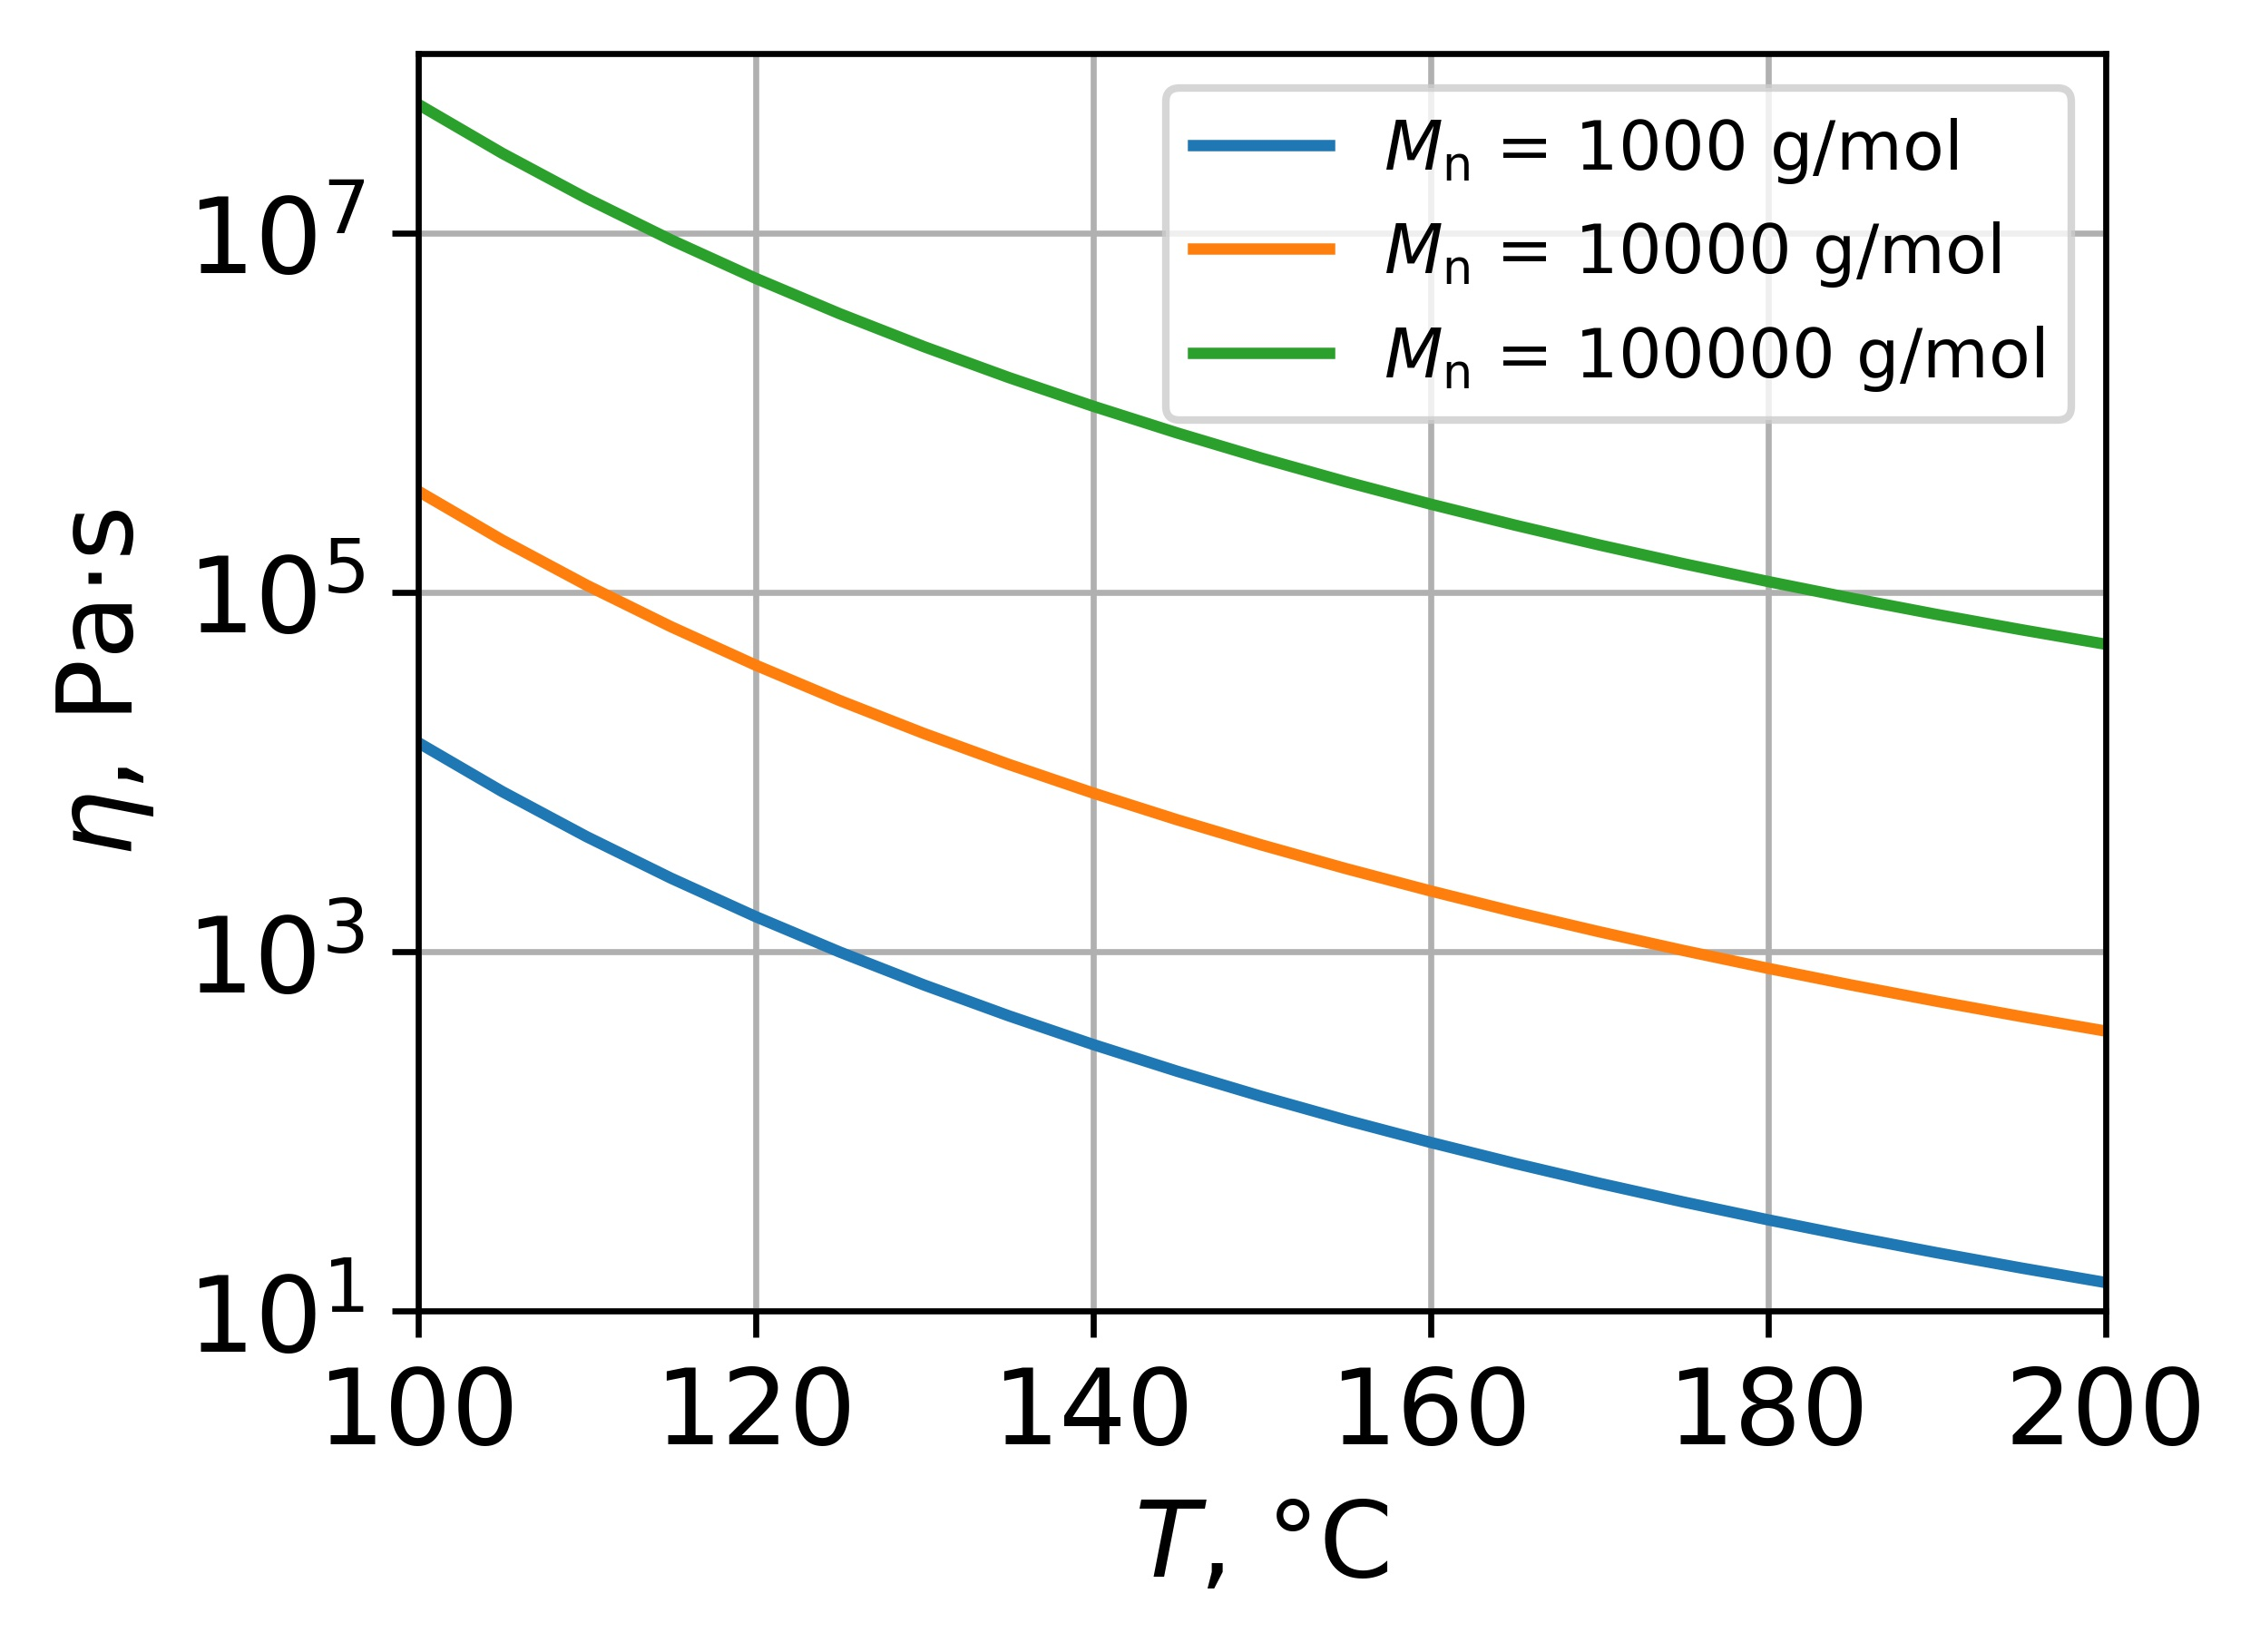
\includegraphics[width=0.5\linewidth]{eta_vary_T_Mn}
	\end{center}
	\vspace{-2em}
	\caption{Temperature viscosity dependencies for PMMA with different number average molecular weights, obtained by equations~(\ref{eq:WLF}, \ref{eq:3p4_3p1}).}
	\label{fig:eta_vary_T_Mn}
\end{figure}

The second approach, numerical one, is based on search of minimal surface by finite elements method. It can be processed by free software ``Surface Evolver'' (SE) -- the program for the modelling of liquid surfaces shaped by various forces and constraints~\cite{Brakke_SE}. SE allows a wide spectrum of possible energies to be assigned like gravitational energy, surface energy, and further different implementations of mean and Gaussian curvature. For the purpose of polymer reflow simulation only surface energy should be taken into account.

In SE simulation algorithm the structure is only described by its ``outer shell'' (soapfilm modeling)~(Fig.~\ref{fig:SE_basic}a)). For the resist reflow simulation the resist surface is divided into triangle facets defined by vertices $v_0$, $v_1$ and $v_2$ and oriented edges $\vec{e_0}$, $\vec{e_1}$ and $\vec{e_2}$, and the polymer reflow is simulated by moving of facet vertices, maintaining the constant volume inside the surface. The force on vertex $v_0$ (the tail of vector $\vec{e_0}$) is

\begin{equation}
	\vec{F}_{v_0}=\frac{\gamma_i}{2} \cdot \frac{\vec{e}_1 \times\left(\vec{e}_0 \times \vec{e}_1\right)}{\left\|\vec{e}_0 \times \vec{e}_1\right\|},
\end{equation}
where $\gamma_i$ -- is surface tension of $i$-th facet~(Fig.~\ref{fig:SE_basic}b)). SE could be operated in the area normalization mode to approximate a vertex motion by mean curvature, i.e., a surface tension flow. In this mode, the velocity of a vertex is proportional to force and indirectly proportional to the area of the facets surrounding this vertex. The $i$-th facet has three vertices associated with it, therefore the relative area contribution to the force of one vertex is 1/3 the area of the surrounding facets $A$. The vertex velocity in the area normalization mode is

\begin{equation}
	\vec{v} = \frac{\vec{F}}{A/3} \cdot \mu,
\end{equation}
where $\mu$ is so called vertex mobility. The vector of vertex movement $\vec{\delta}$ is then calculated as product of vertex velocity and \textit{scale} factor $s$, the physical representation of simulation step time:

\begin{equation} \label{eq:SE_delta}
	\vec{\delta} = \vec{v} \cdot s.
\end{equation}

\begin{figure}[t]
	\begin{minipage}{0.58\textwidth}
		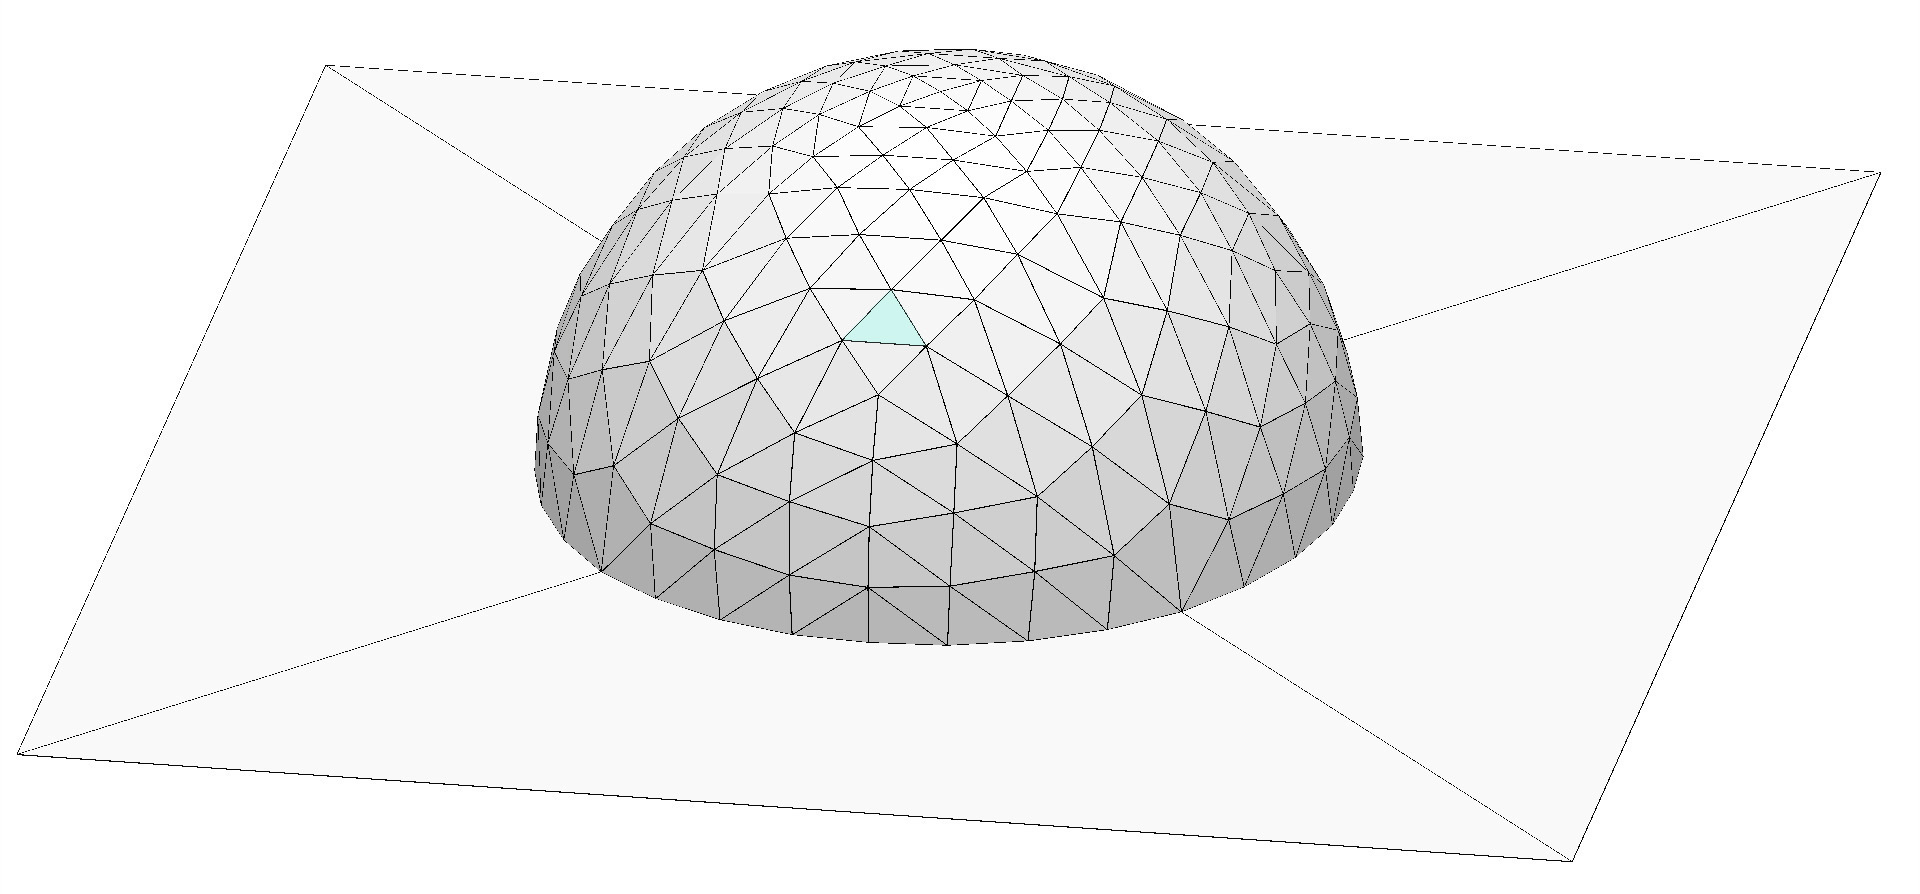
\includegraphics[width=\linewidth]{SE_surface} \\
		\vspace{-10em} \\ \hspace{0em} a) \\ \vspace{10em}
	\end{minipage}
	\begin{minipage}{0.38\textwidth}
		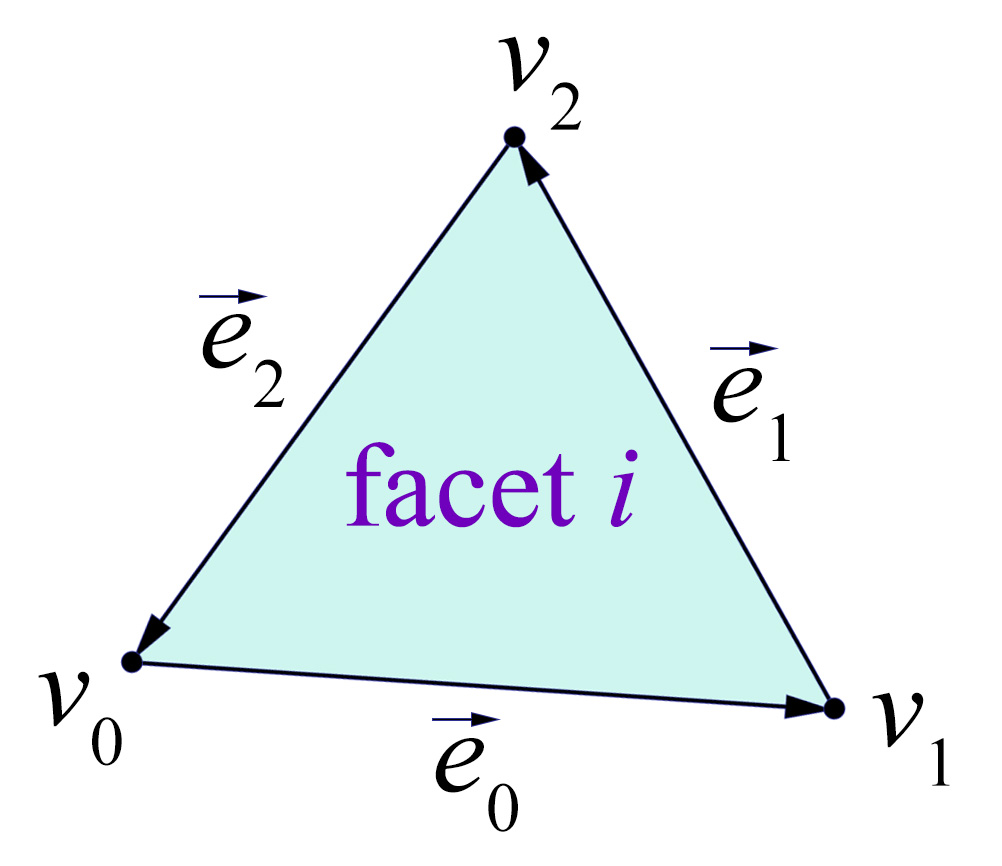
\includegraphics[width=\linewidth]{SE_facet} \\
		\vspace{-10em} \\ \hspace{-0.1em} b) \\ \vspace{10em}
	\end{minipage}
	\vspace{-4em}
	\caption{a) A mound of liquid sitting on a tabletop with gravity acting on it, defined by its surface in SE, b) definition of vertices and oriented edges for $i$-th facet in SE.}
	\label{fig:SE_basic}
\end{figure}


In most cases SE is used just for calculation of minimal energy geometries, which doesn't imply simulation of liquid or polymer flow dynamics~\cite{SE_example_1, SE_example_2}. However, Kirhner~\cite{Kirchner_SE_1, Kirchner_SE_2} demonstrated the applicability of this method for the reflow simulation of step structure, which consisted of two regions with different molecular weight. The difference in viscosity values of regions was taken into account by setting different vertex mobilities. Kirchner showed that mobility ratios 1:2, 1:5 and 1:50 allow to describe structure reflow stages with high accuracy. Mobility ratios were determined empirically, by the comparison of experimental and simulated profiles. In this case, the simulation algorithm is only applicable for the structures obtained with the same exposure doses, and reflow simulation of any other structures require preliminary measurements. On the other hand, the only question in case of any structure reflow simulation operated by SE is the distribution of structure vertex mobilities (neglecting the edge effects). Kirchner mentioned that inverse mobility is a kind of sample viscosity, but the correlation between mobility and viscosity was still unclear. Thus, the purpose of this study is to investigate the relation between polymer viscosity and mobility of its surface vertices and to develop the numerical simulation method for non-uniform resist thermal reflow, using SE as a calculation engine.
